\documentclass[journal]{vgtc}                % final (journal style)
% \documentclass[review,journal]{vgtc}         % review (journal style)
%\documentclass[widereview]{vgtc}             % wide-spaced review
%\documentclass[preprint,journal]{vgtc}       % preprint (journal style)

%% Uncomment one of the lines above depending on where your paper is
%% in the conference process. ``review'' and ``widereview'' are for review
%% submission, ``preprint'' is for pre-publication, and the final version
%% doesn't use a specific qualifier.

%% Please use one of the ``review'' options in combination with the
%% assigned online id (see below) ONLY if your paper uses a double blind
%% review process. Some conferences, like IEEE Vis and InfoVis, have NOT
%% in the past.

%% Please use the ``preprint''  option when producing a preprint version
%% for sharing your article on an open access repository

%% Please note that the use of figures other than the optional teaser is not permitted on the first page
%% of the journal version.  Figures should begin on the second page and be
%% in CMYK or Grey scale format, otherwise, colour shifting may occur
%% during the printing process.  Papers submitted with figures other than the optional teaser on the
%% first page will be refused. Also, the teaser figure should only have the
%% width of the abstract as the template enforces it.

%% These few lines make a distinction between latex and pdflatex calls and they
%% bring in essential packages for graphics and font handling.
%% Note that due to the \DeclareGraphicsExtensions{} call it is no longer necessary
%% to provide the the path and extension of a graphics file:
%% 
\includegraphics{diamondrule} is completely sufficient.
%%
\ifpdf%                                % if we use pdflatex
  \pdfoutput=1\relax                   % create PDFs from pdfLaTeX
  \pdfcompresslevel=9                  % PDF Compression
  \pdfoptionpdfminorversion=7          % create PDF 1.7
  \ExecuteOptions{pdftex}
  \usepackage{graphicx}                % allow us to embed graphics files
  \DeclareGraphicsExtensions{.pdf,.png,.jpg,.jpeg} % for pdflatex we expect .pdf, .png, or .jpg files
\else%                                 % else we use pure latex
  \ExecuteOptions{dvips}
  \usepackage{graphicx}                % allow us to embed graphics files
  \DeclareGraphicsExtensions{.eps}     % for pure latex we expect eps files
\fi%

%% it is recomended to use ``\autoref{sec:bla}'' instead of ``Fig.~\ref{sec:bla}''
\graphicspath{{figures/}{pictures/}{images/}{./}} % where to search for the images

\usepackage{microtype}                 % use micro-typography (slightly more compact, better to read)
\PassOptionsToPackage{warn}{textcomp}  % to address font issues with \textrightarrow
\usepackage{textcomp}                  % use better special symbols
\usepackage{mathptmx}                  % use matching math font
\usepackage{times}                     % we use Times as the main font
\renewcommand*\ttdefault{txtt}         % a nicer typewriter font
\usepackage{cite}                      % needed to automatically sort the references
\usepackage{tabu}                      % only used for the table example
\usepackage{booktabs}                  % only used for the table example
\usepackage{tabularx}
%% We encourage the use of mathptmx for consistent usage of times font
%% throughout the proceedings. However, if you encounter conflicts
%% with other math-related packages, you may want to disable it.

%% In preprint mode you may define your own headline. If not, the default IEEE copyright message will appear in preprint mode.
%\preprinttext{To appear in IEEE Transactions on Visualization and Computer Graphics.}

%% In preprint mode, this adds a link to the version of the paper on IEEEXplore
%% Uncomment this line when you produce a preprint version of the article 
%% after the article receives a DOI for the paper from IEEE
%\ieeedoi{xx.xxxx/TVCG.201x.xxxxxxx}

%% If you are submitting a paper to a conference for review with a double
%% blind reviewing process, please replace the value ``0'' below with your
%% OnlineID. Otherwise, you may safely leave it at ``0''.
\onlineid{0}

%% declare the category of your paper, only shown in review mode
\vgtccategory{Research}
%% please declare the paper type of your paper to help reviewers, only shown in review mode
%% choices:
%% * algorithm/technique
%% * application/design study
%% * evaluation
%% * system
%% * theory/model
\vgtcpapertype{please specify}

%% Paper title.
\title{AsylumLoupe: EU Asylum Demographics and Movement Information Visualization}

%% This is how authors are specified in the journal style

%% indicate IEEE Member or Student Member in form indicated below
\author{Han Wang and Xin Wang}
\authorfooter{
%% insert punctuation at end of each item

\item 
 All authors contributed equally to this work.
\item
 Han Wang, E-mail: whan2019@student.ubc.ca.
\item
 Xin Wang, E-mail: wangxin0@student.ubc.ca.
}

%other entries to be set up for journal
% \shortauthortitle{Biv \MakeLowercase{\textit{et al.}}: Global Illumination for Fun and Profit}
%\shortauthortitle{Firstauthor \MakeLowercase{\textit{et al.}}: Paper Title}

%% Abstract section.
\abstract{In this article we present AsylumLoupe, an information visualization tool with an interactive design, which shows the evolution of asylum applications and resettlement in European countries over time since 2008. By combining the features of the origin destination map and the chropleth map, AsylumLoupe gives the user an overview of asylum-related data for European countries using color and saturation channels. By clicking, dragging, zooming in and out of our interactive map, users can select specific asylum seekers' destination countries and origin countries to customize their exploration. Using different charts, AsylumLoupe shows asylum application and placement data grouped by different attributes respectively, which allows users to compare the number of asylum applicants and granted resettlement for asylum seekers with different attributes (e.g. gender, age, country of origin) in a particular destination country, and trends over time. These information is critical for policymakers to address the social and economic impacts of a migration problem such as refugee crisis in 2015 and help them make changes faster.} 
% end of abstract

%% Keywords that describe your work. Will show as 'Index Terms' in journal
%% please capitalize first letter and insert punctuation after last keyword
\keywords{Asylum, EU, Refugees, Information Visualization}

%% ACM Computing Classification System (CCS). 
%% See <http://www.acm.org/class/1998/> for details.
%% The ``\CCScat'' command takes four arguments.

% \CCScatlist{ % not used in journal version
%  \CCScat{K.6.1}{Management of Computing and Information Systems}%
% {Project and People Management}{Life Cycle};
%  \CCScat{K.7.m}{The Computing Profession}{Miscellaneous}{Ethics}
% }

%% Uncomment below to include a teaser figure.
\teaser{
  \centering
  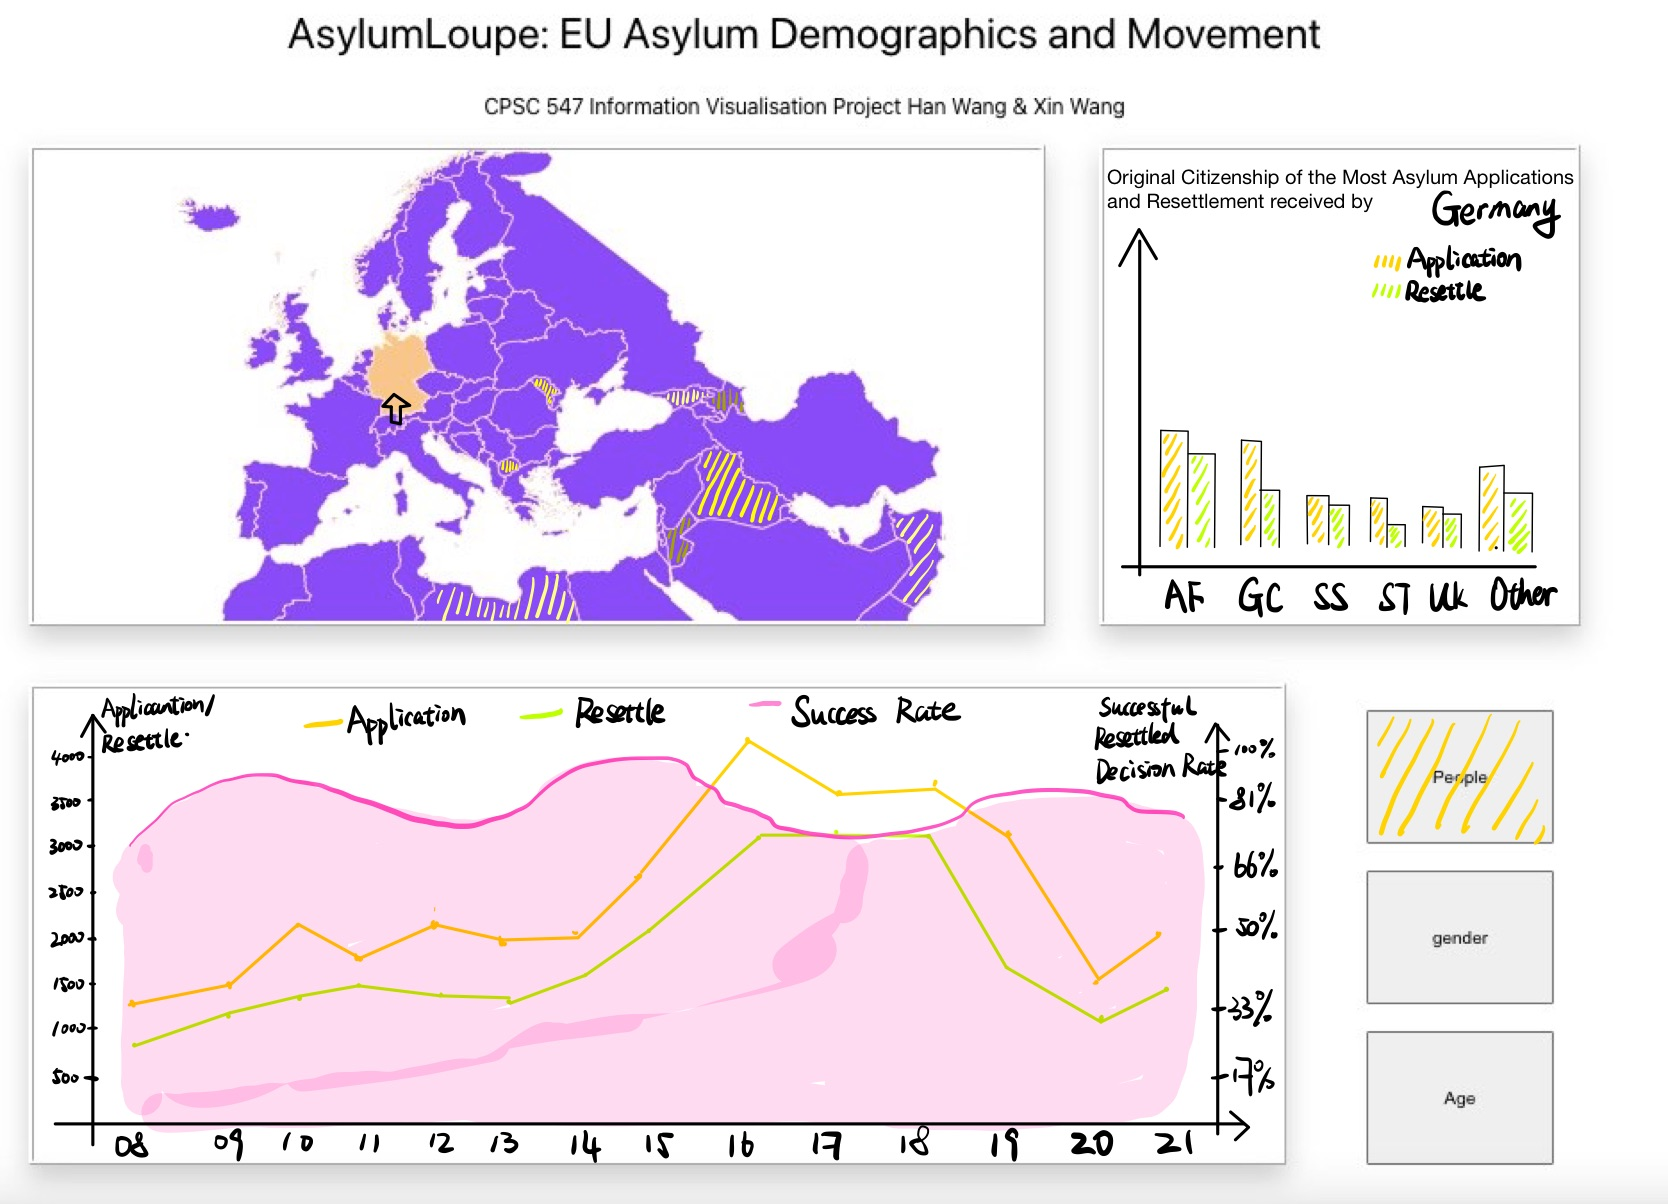
\includegraphics[width=\linewidth]{Sketches-1}
  \caption{AsylumLoupe interface, showing incoming asylum applicants and resettlement receivers in Germany between 2008 and 2022.}
	\label{fig:teaser}
}

%% Uncomment below to disable the manuscript note
\renewcommand{\manuscriptnotetxt}{}

%% Copyright space is enabled by default as required by guidelines.
%% It is disabled by the 'review' option or via the following command: \nocopyrightspace

\vgtcinsertpkg
\nocopyrightspace
%%%%%%%%%%%%%%%%%%%%%%%%%%%%%%%%%%%%%%%%%%%%%%%%%%%%%%%%%%%%%%%%
%%%%%%%%%%%%%%%%%%%%%% START OF THE PAPER %%%%%%%%%%%%%%%%%%%%%%
%%%%%%%%%%%%%%%%%%%%%%%%%%%%%%%%%%%%%%%%%%%%%%%%%%%%%%%%%%%%%%%%%

\begin{document}

%% The ``\maketitle'' command must be the first command after the
%% ``\begin{document}'' command. It prepares and prints the title block.

%% the only exception to this rule is the \firstsection command
\firstsection{Introduction}

\maketitle

%% \section{Introduction} %for journal use above \firstsection{..} instead
The war in the Middle East, the oil crisis, and geopolitical issues have all caused many people to be displaced. Despite continued COVID-19 measures, the number of arrivals to Europe's external borders increased in 2021, returning to pre-pandemic levels. Adapting quickly, EU+ countries (the European Union, Israel, Norway, Serbia, Turkey, and the United Kingdom) facilitated asylum application lodgings, rearranged reception facilities, and used arrival centers for various stages of asylum procedures in response to the waves of arrivals\cite{euaa:2022}. These developments have also highlighted the need for structural reforms of the EU's asylum and migration system to address both crises and longer-term trends\cite{hurwitz:2009}. The existing asylum procedure has been developed from each stage, and the process has been digitized recently as well, including procedures for first and second applications, special procedures, the Dublin procedure, reception conditions, detention during the asylum procedure, access to the asylum procedure and information, legal assistance, interpretation services, country of origin information, the content of protection, the return of former applicants and resettlement. The Dublin procedure establishes the criteria to determine which Member State is responsible for examining an application for international protection. It is a Europe-wide procedure that follows the same criterion for determining responsibility applied similarly in all Member States. There are differences in national legislation and organizational set-ups of Member States, which is why diverse national practices exist when applying the regulation. 

Identifying and monitoring trends in asylum applicants and country of origin countries can be accomplished through the key indicators presented\cite{euaa:2022}. The EU has always been welcoming to refugees, and even before the 2015 refugee crisis, the EU asked its members to submit a series of refugee-related data, which can be found on the Eurostat, which is the statistical database of the European Union to provide high-quality statistics and data on Europe. This database details the number of refugee applicants, temporary asylum seekers, and long-term asylum seekers by age, gender, and nationality since 2008. The European Council committed in 1999 to develop a Common European Asylum System (CEAS) that applies the Geneva Convention fully and inclusively. For the CEAS to develop in the right direction, a period of reflection was required after the first phase. There were still too many differences across EU Member States, and protection levels were still insufficient. As a result of this, the European Commission presented its Asylum Policy Plan in June 2008, which laid the foundation for a system of common and uniform protection standards. In that case, we will use this data from 2008 to 2021 to develop Vis to show and analyze many issues. 

The primary objective of this project is to provide an overview of the refugee intake trends across 27 EU member countries. We also want to present the different distribution of asylum applications, temporary asylum, and long-term asylum across EU member states, and the differences between countries of origin, gender, and age of asylum seekers as detailed information. In that case, we propose an explorer tool to support users to figure out the refugee movement trends within the EU as time progresses. It should also be a helpful analysis tool for users to acquire detailed and intuitive information introduced above and compare them by specific years.

To facilitate better planning resources for future asylum seekers, this project may provide a more intuitive and easier way for a user working for specific institutions to explore the movement of asylum applicants compared to searching and analyzing huge amounts of data from data tables and trees layer by layer the detailed explanation will be described in section 3, Data and Task Abstraction.

\section{Related Work}
\subsection{Asylum in Europe and Asylum Demographic Data}
Asylum refers to the international protection offered by a country on its territory. It is provided for people who cannot seek protection in their own country of citizenship and/or residence, especially those who fear persecution based on race, religion, nationality, wars, membership in a particular social group, or political opinion\cite{unhcr:2012}. This paper presents a information visualization (Vis) project concerning asylum seekers and resettlement in the European Union. Processing asylum applications and resettlement is covered by the EU migration policy. The EU has a long history of regulating its immigration policy, and since the 1951 Convention Relating to the Status of Refugees\cite{the_european_commission:2022}, the EU has continued to improve its migration policy, establishing the current harmonized legislative framework on asylum based on the Treaty on the Functioning of the European Union and the EU Charter of Fundamental Rights as its legal foundation. Each year, the EU makes effort to develop an effective European migration and asylum policy in response to large numbers of migrants coming to the EU resulting from migration crises like the one in 2015\cite{consilium:2022}. The creation of a migration and asylum policy and its operation is based on collecting data on the current situation. An example is the demographic data related to asylum application and resettlement in the EU discussed in this project. 

Eurostat (European Statistical Office), which provides statistical information to the institutions of the European Union, persists datasets related to EU asylum application and resettlement. In terms of presenting these data, Eurostat used a range of published charts with pre-defined data types derived from the dataset of asylum demographics. Eurostat provides a data visualization tool that is integrated into its powerful Eurostat Data Browser\cite{data_browser_eurostat:2020}. For each new dataset published, Eurostat presents the data in the Vis idioms of tables, graphs, and maps on its web page. The Eurostat also integrates the Data Explorer tool, a feature that presents the charts as a search tree. Users can click on a search tree branch to display different charts. While supporting the functionality that current tool provided, the new data browser also adds additional functionality for viewing data and metadata: users can filter data dimensions and adjust the way graphical data is displayed (line, bar, and map charts), which makes it easy to compare indicators and geographical areas\cite{wiki_eurostat:2022}. 
\subsection{Information Visualization Design}
We want to build Vis idioms showing the demographics and movements of asylum application and resettlement in the EU. We need to represent the movement of asylum applicants and resettled refugees by showing the association between known geographic pairs, such as refugees drifting from a country at war, to an EU country seeking asylum. The O(Origin)D(Destination) Map is a good solution for this. OD Map shows the relationship by mapping the geographic vectors between the origin and destination as cells rather than lines. It preserves the spatial layout of OD, and when we need to show multiple “origins” of the “destination” country, e.g., an EU country receiving asylum applications from people in multiple countries, the OD Map does not suffer from the occlusion problems of other solutions, or the loss of detail due to aggregation\cite{slingsby:2010}. Choropleth map utilizes the color channel in corresponding to an aggregated summary of geographic characteristics within spatial enumeration units\cite{dent:1990}, it can visualize how an attribute from our dataset varies across the geographic area. In our case, the choropleth map can contribute to showing the different magnitudes of an attribute in our dataset encoded by saturation and the color channel. Stacked bar charts can help us make more complex data comparisons. A stacked bar chart is a form of bar chart that follows the horizontal coordinates to show the composition and comparison of multiple variables. After selecting the source and destination countries, our Vis will provide comparisons of demographic data, such as comparisons of asylum application, and resettlement numbers by gender, age group, and other ordinal or categorical characteristics. Stacked bar charts allow us to show how these comparisons have changed over time\cite{donnelly_kelley:2013}.

\section{Data and Task Abstraction}

\subsection{Domain}

This Vis project focuses on illustrating the movement and analyzing the demographic data of asylum application and resettlement across Europe, the Middle East, and North Africa (MENA) region from 2008 to 2021. We want to combine credible and rich data in an interactive format to dynamically show the movement of  asylum applicants and resettled refugees in the same time period. Based on this, we will also explore different trends in combination with their demographic data. Our project helps EU policymakers to understand the movement of asylum applicants, explore the changing trends of asylum seekers’ demographic over time, and develop corresponding policies on asylum seekers or refugees, predict the future increase or decrease of asylum seekers in the EU. People in each EU country can also use our project to learn about the asylum demographics in their own country, such as age, gender and original nationality. Therefore, they can learn about domestic asylum with real data, which helps society to eliminate prejudice against asylum receivers and refugees. 

\subsection{Tasks Abstraction}

The biggest task of this project in terms of Vis is to show the movement of asylum applicants,  and resettled refugees in the Europe and MENA region from 2008 to 2021, including their countries of origin and destination. Users can explore the correlation and distribution of asylum applicants and resettled refugees with different age classes, gender classes, and original nationalities across the EU countries. They can also compare the asylum application intake and resettled decisions of the applicants between each year from 2008 to 2021, and find the correlation between successful resettled decisions for asylum applications and different EU countries. On top of this, the project will also select associations between origin countries and  one EU country that has asylum application or resettlement intake. In the case of both origin and destination countries are selected, the distribution of age class, gender class, and original nationality will be presented to allow the reader to identify different patterns and trends. The user can specify different attributes to observe the distribution of these attributes in different classes from 2008 to 2015 and explore the correlation between attributes like age or gender classes and the successful resettled decision in each year.

\subsection{Data Abstraction}
Data for this project are sourced from Eurostat. We selected the annual aggregated data series on asylum applications and resettlement containing statistical information based on Article 4 of the Council Regulation (EC) No 862/2007 from 2008 to 2021. We didn’t adapt the historic data before 2008. The Council Regulation (EC) No 862/2007 concluded the regulation for collecting and analyzing information on migration and asylum in the EU, which included several important changes designed to improve the completeness and degree of harmonization of these statistics\cite{eur_law:2007}. To avoid massive inconsistent data entries, we only sample the dataset referencing this regulation starting from 2008.

Our final dataset will be obtained by concatenating 2 related datasets, the dataset for asylum applicants in all EU member countries and resettlement decision in all member countries from 2008 to 2015. As of today, we worked with more than 1,000,000 items. Each item represents the status of one asylum application or resettlement with reference to different age classes, gender classes, and original citizenship. The national Ministries of Interior and related official agencies provide these data to Eurostat. Data is presented by country and for groups of countries: the European Member States and the European Free Trade Association (EFTA). The attributes we intend to use in our analysis are both categorical and ordered. Dataset is constantly updated\cite{european_commission:2021}. We selected the newest latest dataset on 13th November 2022. Specifically, the levels of categorical attributes are as shown in \autoref{tab:lev1}. The ranges for ordered attributes are listed in \autoref{tab:lev2}. One example item/data entry from the origin datasets is presented in the \autoref{fig:tab3}.

\begin{table}[]
  \caption{Level of Categorical Attributes for EU Asylum Application and Resettlement Dataset - Annual Aggregated Data}
  \label{tab:lev1}
  \scriptsize
	\centering
  \begin{tabularx}{\columnwidth}{XXXX}
    \toprule
    Dimensions[code] & Levels & Labels[code] & Note \\
    \midrule
    Time-Frequency [FREQ] & 1 & Annual[A] & Only annual data included \\
    Country-of-Citizenship [CITIZEN] & 208 & Countries, or regions defined by Eurostat represent by ISO 3166-1 alpha-2 country codes. & We cleaned the data, only Europe and MENA countries and regions remain in final dataset. \\
    Sex [SEX] & 4 & Total [T], Males [M], Females [F], Unknown [UNK] & [T] equals the sum of [M], [F] and [UNK]. \\
    Application-Type [asyl\_app] & 3 & Asylum-Applicant [ASY\_APP], First-Time-Applicant [NASY\_APP], Subsequent-Applicant [SSEQ] & [ASY\_APP] equals [NASY\_APP] plus [SSEQ], asylum application dataset only. \\
    Unit of Measure [unit] & 1 & Person [PER] & \\
    Geopolitical Entity [geo] & 34 & 33 geo political entities in EU plus European Union of 27 member states [EU27\_2020] & Geo political entities include the EU, EEA(European Economic Area), EFTA countries, exit members included.
  \end{tabularx}
\end{table}

\begin{table}[]
  \caption{Range of Ordered Attributes for EU Asylum Application and Resettlement Dataset - Annual Aggregated Data}
  \label{tab:lev2}
  \scriptsize
	\centering
  \begin{tabularx}{\columnwidth}{XXX}
    \toprule
    Dimensions[code] & Range[code] & Note \\
    \midrule
    Age Class [Age] & Total [Total], Less than 14 [Y\_LT14], From 14 to 17 [Y14-17], Less than 18 [Y\_LT18], From 18 to 34 [Y18-34], From 35 to 64 [Y35-64], 65 or older [Y\_GE65], Unknown [UNK] & Age of the applicants are distributed into 8 classes, some countries didn't split the class under 18. \\
    Time [Time] & From 2008 to 2021 & Each year represents an attribute. \\
    Cell value & From 0 to 1216806 & Value of each year, represents the number of applications or resettlements. \\
  \end{tabularx}
\end{table}

\begin{figure}[tb]
  \centering % avoid the use of \begin{center}...\end{center} and use \centering instead (more compact)
  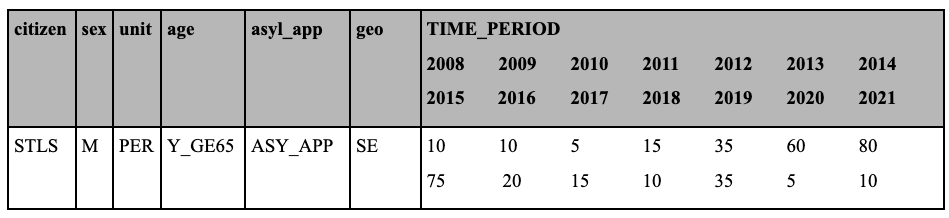
\includegraphics[width=\columnwidth]{tab3.png}
  \caption{Example Data Entry for EU Asylum Application Dataset - Annual Aggregated Data}
  \label{fig:tab3}
 \end{figure}

We filtered out the “Time of Frequency” and “Unit of Measure” attributes, which have the same value in each entry and contain no additional information. We also filter out certain levels or ranges for the different attributes, and the specific information is summarized in the note column on the right of each table. We cleaned the data before implementing the Vis. We used NumPy and pandas libraries in python to eliminate all non-compliant attributes. In the original data, all “Time” attributes were listed in one column, and we separated the “Time” attributes by commas so that each different class of Time was given a separate column. We then align it with other data in the same row to get a valid CSV file. Next, we tackled the non-compliant values, e.g. some of the “Time” attributes have non-integer data in the field, which we change to 0. We use the summation formula to sum the values of all the time attributes of each entry when the value sum of all time attributes is 0, it proves that there is no record of this type of application or resettlement entry, so we also eliminate it. After finishing the data cleaning, we have 87,728 rows of application data and 6908 rows of resettlement data left. \autoref{fig:tab4} lists the sample rows of application/resettlement after completing the cleaning.

\begin{figure}[tb]
  \centering % avoid the use of \begin{center}...\end{center} and use \centering instead (more compact)
  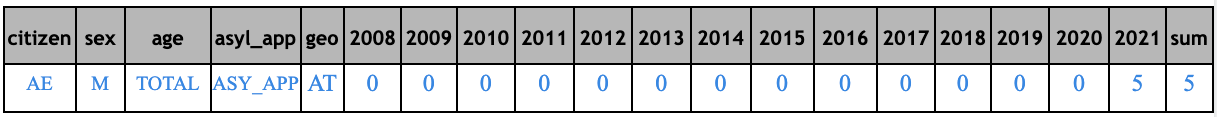
\includegraphics[width=\columnwidth]{tab4.png}
  \caption{Example Cleaned Data Entry for EU Asylum Application Dataset - Annual Aggregated Data}
  \label{fig:tab4}
 \end{figure}

 \section{Solution}

 In the visualization design we propose, there are three interactive views - the origin-destination map view, the insight charts view, and the statistical charts view - for exploring destination and origin-destination countries.
 
 \subsection{Origin-destination map view}
 The origin-destination map, as we discussed previously in section 2.2, allows us to better track asylum applications and resettlements and show the geographic distribution of asylums. Instead of simply using arrows directing from origin countries to destination countries, we choose a choropleth map utilizing motion and color channels as our solution to reduce the direction data.
 For the OD Map view, we use a choropleth map-styled origin-destination map as our solution. In more detail, we display the demographics of destination and origin countries for the number of applications and resettlements using different saturated colors, purple and orange, respectively. The data-driven choropleth map display would help users decide where to click to explore the detailed information.
 There are two manipulations provided for users. One is to zoom in or out of the origin-destination map. The OD Map will initially locate itself in European according to our database. Users can zoom in on the OD Map to see a clearer outline of the country compared to the number of refugees applying or resettling in that country and other countries, thus supporting users to explore refugee movements more effectively. Users can also zoom out to see an overview of the map with more countries to get a sense of the overall refugee application or resettlement situation.
 To show both the refugee application and resettlement statistics on the OD Map, we selected the diverging colormap as our color channel in our solution. We used purple and yellow hues as our two endpoints and a goose yellow colour close to white as our midpoint color. Five degrees of purple are rendered for the destination country and five degrees of orange are rendered for the origin country. The darker the colour, the more refugees are accepted for application or processed for resettlement in that country, and vice versa. When selecting one of the destination countries, the origin countries where the applications received by the destination countries come from will be immediately filled in orange with different saturation according to the number of applications.
 To highlight the selected destination country, we use dark purple as its color. Similarly, if the user chooses an origin country, that country will also be highlighted using dark orange. The direction from orange to purple countries indicates the refugee movements. In the absence of applications or resettlements, the color will be gray for a specific country. Besides, we also provide a tooltip for users to get to know the application or resettlement numbers and destination country names.
 \subsection{Insight charts view}
 The insight charts view contains two pages, one is the Sankey chart and the other is the pie charts as our solution. We use an insight charts view to help users better explore the OD Map view. Before a destination country is selected, the insight charts view will offer users some guidance to help them better explore the OD Map at the start.
 After a destination country is selected, the insight chart on the left-hand side shows a Sankey chart with two parts, the number of applications and resettlement respectively, which help users to acquire an intuitive insight into the difference between the number of applications and resettlement.
 The Sankey chart shows the top five countries with the highest number of applications submitted to the selected destination country. We can also see the detailed application and resettlement number through the tooltip as well. One link between the insight charts view and the OD Map view is the same country name shown on both two views. The other is that we use the same color channel with a diverging color map for both views. We use the diverging red to green colormap to correspond to the top five origin countries with the most asylum applications for the destination country, from most to least, which corresponds to the dark to light purple or orange color channel in the OD Map.
 We initially used a bar chart with a scatterplot to represent the application and resettlement data for a specific country inside the same insight charts view page for a better comparison. Even after processing by mapping or taking logarithms or scaling orders of magnitude, the number of applications and resettlement cannot both be presented well in the same chart due to the large difference between the number of asylum applications and the number of applications granted in the same country. In that case, to show both application and resettlement data, as well as the difference between them, we choose a Sankey chart to show the data without extra processing.
 After selecting the origin country, the insight charts view will change to another page to show the pie chart. We chose the pie chart as our solution to show the ratio of applications from the origin country to the total number of applications accepted in the destination country, so as the ratio of approved applications from the origin country to the total number of resettlement approved in the destination country. In the insight charts view, the destination countries are shown in green and the source countries are shown in blue, corresponding to the destination countries in dark purple and the origin countries in dark orange in the OD Map, respectively. Besides, another link is also the same country name inside the tooltip as we mentioned before.
 \subsection{statistical charts view}
 With the overview information provided by the OD Map view and the insight charts view mentioned before, we also need detailed information to help users make a better exploration. To present data with more specific details, we choose to reduce the data by filtering it by different attributes of the data entry, including “people”, “gender” and “age” pages and display the data using the double-bar chart, the line chart and the stacked bar chart respectively in the statistical charts view as our solution.
 Because we found that the data range between some age groups and gender groups is different from each other, which affects the overall display, and sometimes the stacking of lines and bars is not conducive to the accurate reading of information, we adopt logarithmic mapping for the data in the statistical charts view as a whole. After the above processing, we can display the data with more details through reasonable scaling, so that users can get more detailed information from our visualization tool.
 We choose a double-bar chart for the “people” page as our solution. We use the group bar to aggregate the number of applications and resettlement by year from 2008 to 2021 for easy comparison by the user. Based on the colour channel, we use blue for the number of applications and green for the number of resettlement. The chart is still linked to the OD Map by showing the name of the selected country. Depending on whether the user selects the destination country or the origin country, the chart's presentation changes accordingly. The maximum and minimum values are specially marked with an accurate number, and the blue and green dotted lines indicate the average of applicants and resettlement respectively in the past years from 2008 to 2021. Users can see more detailed information using the tooltip as well.
 When the user selects only the destination country, the chart shows the number of refugee resettlement and applications in the destination country regardless of their citizenship. When the user selects both destination and origin countries, the chart shows the number of asylum applications submitted from the origin country to the destination country and the number granted from 2008 to 2021.
 For the “gender” page, to better focus on the gender types, we grouped the data with applications and resettlements to reduce other attributions. In the line chart, we used six lines of different colors based on a categorical colormap to represent each of the six genders of asylum applicants. The link to the OD Map still relies on the name of the countries displayed.
 Similarly to the \"people\" page, when the user selects only the destination country, the chart shows the annual refugee resettlement and application gender data in the destination country regardless of their citizenship. When the user selects both destination and origin countries, the chart shows the number of asylum applications submitted from the origin country to the destination country and the number granted grouped by gender from 2008 to 2021.
 For the “age” page, we use a stacked bar chart as our solution to show the application and resettlement data for 8 age groups per year over the past 14 years. Stacked bar charts allow users to compare annual data between different age groups more visually than line charts. The attributes are reduced by grouping the application and resettlement numbers together. We also used a categorical colormap to represent data in 8 groups with different colors. The link to the OD Map still relies on the name of the countries displayed.
 Similarly to the \"people\" page, when the user selects only the destination country, the chart shows the annual refugee resettlement and application age data in the destination country regardless of their citizenship. When the user selects both destination and origin countries, the chart shows the number of asylum applications submitted from the origin country to the destination country and the number granted grouped by age from 2008 to 2021.
 \section{Results}
 \subsection{User Scenario 1}
 For the destination countries, which are EU+ countries, where refugee asylum applications are processed, refugee service agencies would like to assess whether basic services such as infrastructure, service personnel, and service types need to be improved by analyzing specific data in a certain year since EU+ countries aim to provide continuously improved services for asylum seekers. The first user scenario is that EU+ countries handle asylum applications and make decisions on resettlement. For example, analyzing and improving the configuration of the number of different language service providers based on the asylum application data flowing into the destination country through the visualized data in the view. Another example is to increase or decrease the infrastructure required for a specific age group through the asylum application age visualization displayed on the “age” page of the statistical charts view. Or users can use this vis tool to ensure fairness to refugees from different countries by adjusting the number of asylum applications approved in the destination country with the help of the insight view. 
 As shown in Figure 1, The immigration officer from one EU+ country, for instance, Germany wants to compare the asylum statistic between 2008 and 2021 to explore the correlation between asylum applicants and their original citizenship. Along with time progress, the officer wants to know people from which countries or regions sent the most asylum applications to Germany and from which country or regions have the highest possibility to receive a resettled decision, then the officer can explore the insight charts view along with the OD Map view to get an intuitive insight. The officer could also compare the total number of asylum applicants and resettlement between different years, if a growing trend is explored, the officer could allocate more resources to asylum matters or call for help from other member states through the visualized data provided by statistical charts view.
 \subsection{User Scenario 2}
 For destination EU+ countries where asylum applications are processed, refugee service agencies would like to see a comparison of data for two selected years from 2008 to 2021, to analyze the changes in the number of applications and the trend of the ratio for resettled applicants among all applicants. Although the overview of data from 2008 to 2021 is provided, to make a more customized and clear comparison, refugee service agencies may still need to select two specific years among the 14 to analyze the trend. In that case, the analysis based on the visualized data will help refugee service agencies with their processing speed, work efficiency, and personnel allocation to deal with asylum applications. For example, if the refugee service agencies find out there is an increasing trend in the value between applications and resettlements by comparing the yearly application and settlement grouped bars in the “people” page inside the statistical charts view, they may need to enhance their efficiency of the asylum application processing by some adjustments to meet the increased needs of asylum applicants. For another example, refugee service agencies can judge whether it is necessary to expand refugee shelters based on the trend of the number of asylum applications flowing from the origin country to the destination country by comparing the data between two selected years using the tooltip.
 \section{Future work}
 Firstly, user Testing is important for a visualization tool. However, due to the time limitation, we lack suggestions from real users for improvement in usability and interaction
 Secondly, for the OD Map view, we will try to separate applicants and resettlement data for better visibility and add the corresponding legend to them.
 Thirdly, for the link among the three views, we mainly used the tooltip notice for the same country and the same diverging colormap. It will be more intuitive if we highlight the targeted country.
 
\begin{figure}[tb]
  \centering % avoid the use of \begin{center}...\end{center} and use \centering instead (more compact)
  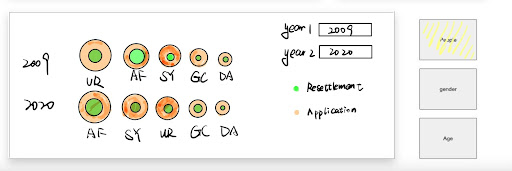
\includegraphics[width=\columnwidth]{fig5}
  \caption{Overview Schematic Diagram for Two Selected Year}
  \label{fig:us2-1}
 \end{figure}

To implement the function of time selection, we have included two time-select menus for users to select different years to make comparisons with. In that case, refugee service agencies are able to determine the trend of refugee movements within the EU over time. 

Besides, this vis also allows the comparison of application and resettlement data between different origin countries where the asylum seekers come from. We use the green color to represent the number of resettled asylum applicants from an origin country. So as the orange color represents the number of applications made from an origin country. The comparison between the number of applications and resettlements for a specific country can be made more intuitively through concentric circles with a certain degree of transparency. When clicking the button “people”, the data will be divided into groups by 5 main origin countries as \autoref{fig:us2-1} shows, and that will be divided into groups by three gender types or four age categories by clicking the button “gender” and “age” respectively. The data will also be sorted based on its quantity among all groups. 


\section{Implementation}
The development of Vis was divided into two parts: the processing of the data and the implementation f the web application. Pandas library in Python are used to analyze and process the data. We first manually cleaned the asylum applicant and placement data downloaded from Eurostat to ensure that it was in the form of a csv file that could be read correctly by Pandas. With this step we divided the data of asylum applicants or resettlement in the rightmost column of the \autoref{fig:tab3} into separate columns by year, as shown in the \autoref{fig:tab4}. Using Pandas we remove the data entries with only 0 values for years 08 to 21, and we also adjust the data entries for different attributes, such as removing data for some controversial countries and regions, as well as some data that are suspected to be wrong. We then used the jq command line tool to convert the CSV file to json. although the front-end framework we were using could accept CSV input, converting to json simplified our code and eliminated potential errors in data I/O.

We picked the ReactJs library as the basic framework for front-end development. Both authors have some basic knowledge of JavaScript, and ReactJs is also suitable for writing single page applications as required by our Vis project. Origin Destination Map was developed by  utilizing the react-simple-maps library, which allowed us to build SVG maps in react with d3-geo and topojson using a declarative api. All other charts are implemented with echarts-for-react library, which is a wrapper integrated in react for creating Vis with Apache E-Charts. We can borrow the rich templates in the E-Chart library and modify them to fit our use case.

\section{Milestones}
Initially we planned to devote 160 hours to this project, and we eventually managed to complete the work as scheduled. The \autoref{tab:share} will provide a detailed explanation of how we allocated our time. Two authors share the responsibility of research, development, implementation and literary write up.

\begin{table*}[b]
  \caption{Share of Work in Project with Estimated and Actual Hours}
  \label{tab:share}
  \scriptsize
	\centering
  \begin{tabular}{p{0.18\linewidth}p{0.5\linewidth}p{0.12\linewidth}p{0.12\linewidth}}
    \toprule
    Task & Description & Estimated Hours/Completion & Actual Hours/Completion \\
    \midrule
    Pitch & Create pitch slides, gather ideas, and write up pitch documents. (All) & 4/Sep. 28 & 4/Sep. 28\\
    \hline    
    Pre-proposal meeting & Retrospect on old pitch idea, finalize topic and create current one. & 4/Oct. 12 & 8/Oct.14 \\
    &Gather datasets from Eurostat.&&\\
    &Write down motivations and possible scenarios, present to Tamara.(All)&&\\
    \hline
    Proposal & Write project proposal.(All) & 4/Oct.21 & 4/Oct.21 \\
    \hline
    Implementation part 1 & Research on suitable tools and Vis Presentation. && \\
    &Clean, abstract, transform and aggregate data. && \\
    &Finish requirement analysis, create user scenarios and scratches. && \\
    &Design and Implement Project baseline application. && \\
    \hline
    Project report update & Write project report update.(All) & 4/Nov. 15 & 4/Nov. 15\\
    \hline
    Peer project review & Prepare demo for project review, get feedbacks from peer and provide to peer projects.(All) & 2/Nov. 16 & 2/Nov. 16 \\ 
    \hline
    Implementation Part 2 & Implement Origin Destination Map. (All) && \\
    & Implement all insights views. && \\
    & Implement all charts and table views. && \\
    & Final touches and refinement on implementation. && \\
    \hline
    Final Presentation & Prepare and rehearse presentation. (All) & 6/Dec. 14 & 6/Dec. 14\\
    \hline
    Final Report & Finish writing final report.(All) & 8/Dec. 16& 8/Dec. 16\\
    \midrule
    \textbf{Total}&&\textbf{160/Dec. 16} & \textbf{160/Dec. 16} \\
    \bottomrule
    
  \end{tabular}
\end{table*}

\section{Results}
\section{Discussion and Future Work}
\section{Conclusions}

In this article we redefine a way to present asylum seeker movement data. By combining the characteristics of the Choropleth map and the origin destination map, we show users the flow of asylum seekers and resettled persons in Europe, while using geographic areas marked with different colors and saturation helps us to compare the quantitative value. In addition to presenting the attribute of number, we also used multiple tables to regroup the data according to different attributes (gender and age groups) and present them separately together with changes over time, which helped users to customize their exploration and better explore the asylum seeker data over time. With the help of further work on linking different views, we can improve the interactivity of Vis. The user can click on, or hovering over  a country on the Map or the insight charts, the corresponding country on the other tables will be selected or highlighted. Together, we give users a more intuitive view of European asylum movement, the general public will have a better understanding of asylum seekers in their countries, and policy makers will be able to make timely changes and improve the immigration system with the help of Vis.


%% if specified like this the section will be committed in review mode
% \acknowledgments{
% The authors wish to thank A, B, and C. This work was supported in part by
% a grant from XYZ (\# 12345-67890).}

%\bibliographystyle{abbrv}
%\bibliographystyle{abbrv-doi}
%\bibliographystyle{abbrv-doi-narrow}
\bibliographystyle{abbrv-doi-hyperref}
%\bibliographystyle{abbrv-doi-hyperref-narrow}

\bibliography{template}
\end{document}

